% TRANSLATION UNIT: translate this file only.
% ===========================================================================
%  09 — Diseño de interfaz y experiencia
%  The \section title is the canonical (Spanish) chapter name; the body prose
%  is written in ENGLISH and translated to Spanish later.
% ===========================================================================

% EVIDENCE INVENTORY (every claim in the prose maps to a real artifact):
% EVIDENCE: one accent #14477A on warm paper #FBFBF9, 880 px content column, 680 px reading column, 2 px radii → frontend/src/styles/tokens/colors.css (--fc-accent, --fc-paper), spacing.css (--content-max, --reading-max), brief §2/§4/§5 (docs/informe/03-brief-diseno.md).
% EVIDENCE: three competing accents (coral, marigold, purple) read as a 2010 portal; hierarchy carried by chrome → docs/informe/03-brief-diseno.md §1, §6.
% EVIDENCE: measured AA ratios 17.15:1 / 7.86:1 / 9.16:1 / 11.40:1; white on accent 9.49:1; white on danger 7.57:1 → frontend/src/styles/tokens/colors.css (inline comments).
% EVIDENCE: AA = 4.5:1 normal text, 3:1 for text >= 24 px or bold >= 19 px → docs/informe/03-brief-diseno.md §2.
% EVIDENCE: design-debt reports 0 artisanal-class screens and 0 inline styles → frontend/scripts/design-debt.mjs --check; completion criterion SC-027 + research D-26.
% EVIDENCE: styles.scss (116 lines, 15 classes) was a partial duplicate of 11 reference components → specs/003-design-system-frontend/research.md:26, spec.md §Contexto.
% EVIDENCE: styles.scss no longer exists → design-debt.mjs reports "eliminado"; plan.md D-26.
% EVIDENCE: 19 primitives exported by shared/ui/index.ts → frontend/src/app/shared/ui/index.ts:1-19.
% EVIDENCE: fc-module, fc-num, fc-linklist survive in tokens/base.css; fc-eyebrow retired → frontend/src/styles/tokens/base.css:140-170; brief §6.
% EVIDENCE: breakpoint tokens 480/768/1024/1280, 1280 a deliberate no-op, 360 px floor → frontend/src/styles/tokens/breakpoints.css.
% EVIDENCE: --page-gutter 20/32/48 px; @media cannot use var() so literal + token comment → spacing.css, breakpoints.css header.
% EVIDENCE: brand panel degrades to a compact band under 768 px and is never hidden (N-14) → frontend/src/app/shared/ui/brand-panel/brand-panel.component.css:130-171; plan.md N-14.
% EVIDENCE: a monetary figure is never truncated (N-15, Principle VIII); truncating $1.234.567 to $1.234… is a false datum → specs/003-design-system-frontend/plan.md N-15; frontend/src/styles/tokens/base.css:120-131 (.fc-num).
% EVIDENCE: result figure drops one type step below 768 px so the full amount fits 320 px; reduce the type, never the datum → frontend/src/app/features/simulators/result/result.component.css:109.
% EVIDENCE: eyebrows 32 -> 0 and three-zone grids 6 -> 1 → aggregated before/after probe recorded in .memory/01a170d5-589e-7520-96bf-71cf23afa320/JOURNEY.md:23 and work-plan.md:67.
% EVIDENCE: 4 px overflow at 360 px on /simuladores/colombia_especifica; 344 px label in a 320 px column → docs/informe/chapters/11-pruebas.tex:21; frontend/src/app/features/simulators/forms/simulator-form.component.css:67; --fc-btn-wrap fix in frontend/src/app/shared/ui/button/button.component.css:54.
% EVIDENCE: contrast regression 3.77:1 on inset surface; 4.38:1 on accent tint vs claimed 4.76:1 measured against white → frontend/src/styles/tokens/colors.css (four-surface table).
% EVIDENCE: e2e selects by role and accessible name in 110 of 112 assertions → getByRole/getByLabel count across frontend/e2e, measured 2026-11-03 (chapters/11-pruebas.tex evidence).
% EVIDENCE: unnamed role="progressbar" announced without a name; fix derives the name from ariaLabel or the visible label → frontend/src/app/shared/ui/progress-bar/progress-bar.component.ts:21-30.
% EVIDENCE: "Regístrate" distinguishable only by color at 1.92:1 (WCAG 1.4.1); fixed by underlining links inside prose → frontend/src/styles/tokens/base.css:84-96.
% EVIDENCE: editorial screen limited to the frame, not the writing surface (FR-123) → specs/003-design-system-frontend/spec.md:365; plan.md Structure.

\section{Diseño de interfaz y experiencia}

\subsection{Institutional calm is a decision under constraint}

The redesign did not set out to decorate. Its target was a specific failure of hierarchy: the
application read like a 2010 web portal because every block carried its own chrome — bordered
module boxes with a three-pixel accent bar, spaced uppercase eyebrows over each title, dotted
separators, a right-hand rail, and three accents competing in one viewport (the coral of the
brand, the marigold of the \enquote{featured} slot, and the purple of links). In that scheme the
hierarchy was carried by borders and tints, and the result was intranet density. The direction
that replaced it is a single sentence: \emph{the hierarchy is carried by typography and space, and
color only signals state or action}.

The chosen form is deliberately sober. One deep blue accent, \texttt{\#14477A}, sits on a warm paper
background, \texttt{\#FBFBF9}, with a reading column of 880 px, a narrower 680 px column for running
text, a maximum radius of 2 px, and no shadow except on genuinely overlaid layers. This is not
taste; it is a decision made under three constraints that any other palette would have failed
just as hard. First, \emph{institutional credibility}: the platform is presented by a university
to a Colombian public-university audience, and a saturated, multi-accent interface would read as a
consumer landing page, not as an instrument a student trusts with money. Second, \emph{long reading
sessions}: the core content is financial-education articles, so the design optimizes a person
sitting through paragraphs, not a person scanning a dashboard. Third, \emph{measurability}: the
brief required every text/background pair to pass AA contrast on the color actually rendered, which
rules out the very gradients and tints that made the old portal busy. A solid accent is the only
thing a contrast checker can measure, because the computed background of a gradient is transparent.

The result is visible in Figure~\ref{fig:login-1280}: the brand panel is a flat blue surface, the
mark is drawn in a single ink, and the form is the only other zone. There is no gradient from coral
to purple, because that gradient was the one place where the three old accents appeared at once.

\begin{figure}[htbp]
  \centering
  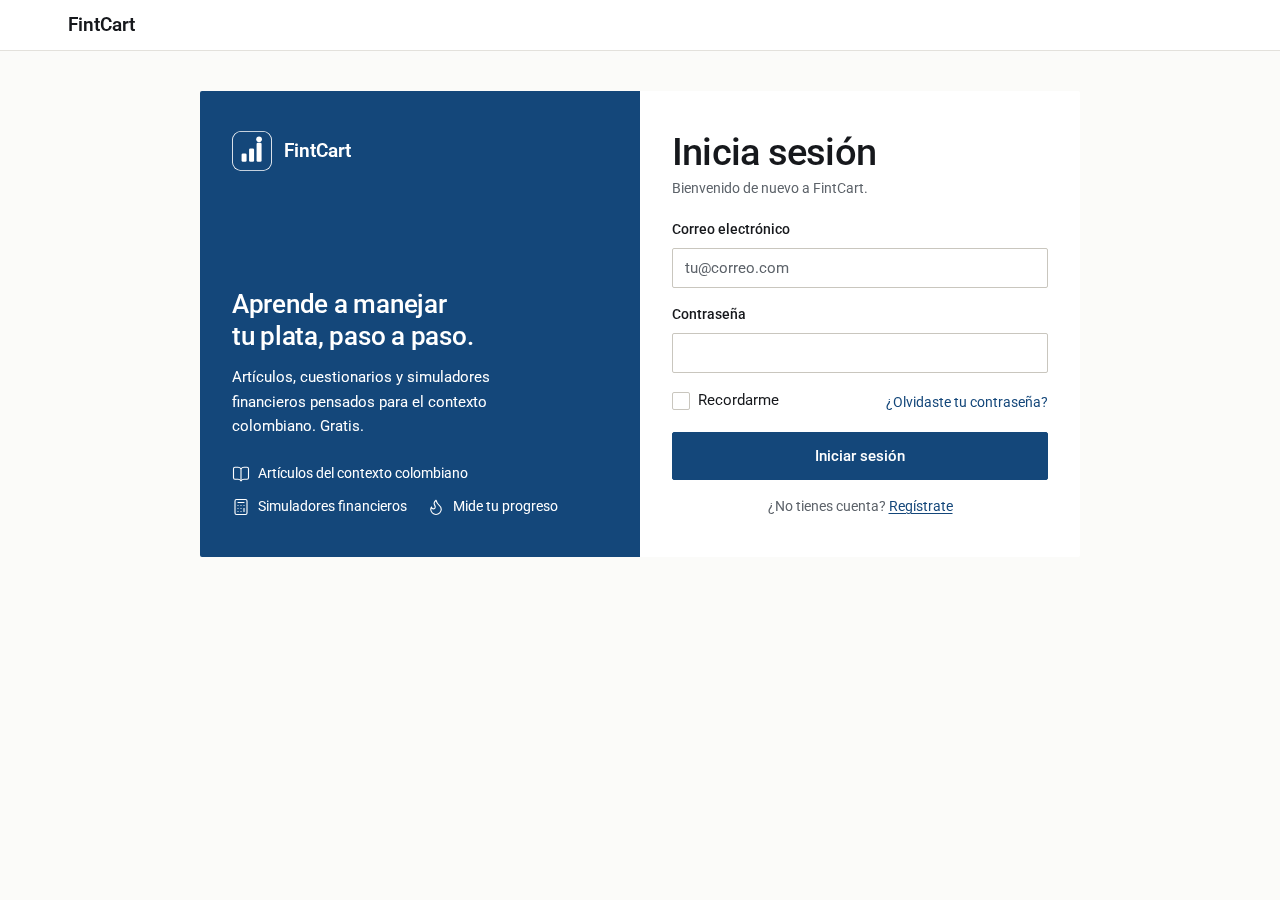
\includegraphics[width=0.72\linewidth]{fig-login-1280}
  \caption{Login screen at 1280 px. The accent is one flat blue, the mark is monochrome on it, and
  the form is the only competing zone — notice that no second accent colors any control.}
  \label{fig:login-1280}
\end{figure}

\subsection{A token layer that can be checked}

The difference between a design system and a stylesheet is that one of them can be checked. A
stylesheet is a set of values someone wrote once; a design system is a set of named values with a
single owner, plus an instrument that fails the build when a screen stops using them. FintCart's
token layer is that owner: \code{colors.css} declares the palette and only the palette,
\code{typography.css} declares the eight type roles as size/height/weight/tracking quartets,
\code{spacing.css} declares the four-pixel grid and the frame measures, and \code{breakpoints.css}
declares the responsive scale. No screen may invent a literal; a screen cites a token, and the
token is where a value is changed exactly once.

The instrument is \code{frontend/scripts/design-debt.mjs}. It scans every screen template and
counts three things: inline \code{style="..."} attributes, references to the retired artisanal
classes (\code{fc-btn}, \code{fc-input} and the rest), and the continued existence of
\code{styles.scss}. Its \code{--check} mode reports zero artisanal-class screens and zero inline
styles, and that number — not a designer's opinion — is the feature's completion criterion
(SC-027). A design system that cannot be checked is just a stylesheet with a nicer name, because
nothing stops the next screen from reintroducing a hex literal and eroding the system by
accretion. Here the erosion is detected at the gate.

\subsection{Nineteen primitives, and a layer retired instead of added}

The instinct when \enquote{the interface looks poor} is to write more styles. That instinct is
exactly what produced the problem this feature exists to remove: the application already had two
layers — the tokens and a hand-made layer in \code{styles.scss}, 116 lines and 15 classes,
commented as \enquote{inspired by} the design system's components — plus 94 inline style
attributes in templates where neither layer reached. The plan therefore did the opposite of the
instinct (design note N-12): it \emph{retired} the artisanal layer and substituted the shared
component library, and it measured progress by what disappeared, not by what was written.
\code{styles.scss} was emptied class by class as each screen group migrated, and it no longer
exists.

What the screens now use is the set of nineteen primitives exported by
\code{shared/ui/index.ts}: \code{fc-button}, \code{fc-input}, \code{fc-select}, \code{fc-checkbox},
\code{fc-card}, \code{fc-module-box}, \code{fc-badge}, \code{fc-tag}, \code{fc-banner},
\code{fc-empty-state}, \code{fc-error-state}, \code{fc-brand-panel}, \code{fc-brand-logo},
\code{fc-progress-bar}, \code{fc-skeleton}, \code{fc-tabs}, \code{fc-icon}, \code{fc-avatar} and
\code{fc-link-button}. Three portal primitives survive in \code{tokens/base.css}, each reduced to
its minimal function: \code{fc-module} is now pure separation between blocks,
\code{fc-linklist} is a silent index of links, and \code{fc-num} is the protected monetary figure.
A fourth, \code{fc-eyebrow}, was retired outright: the spaced uppercase label above every title
was replaced by the title itself.

One distinction had to be written down so that nobody \enquote{fixes} it later: the coral mark was
kept. The redesign's rule was never \enquote{one color in the product} but \enquote{one accent in
the interface}. Coral competed when it was an interface accent — buttons, links, card backgrounds,
category colors — and all of that disappeared. A logo is not an accent; it is the brand. The
sentence that summarizes the decision: \emph{one voice in the interface, one signature in the
brand}. On the blue access panel the mark is drawn white (its inverse variant), which is the
ordinary application of the rule on a dark background, not an exception to it.

\subsection{Responsive with a single scale}

Before this feature, the frontend was not coherently responsive: media queries existed, but the
breakpoints were not unified as tokens and no minimum width was declared. The correction was to
define a single scale and own it in one file. Four breakpoints are declared as tokens —
\code{--bp-sm} at 480 px, \code{--bp-md} at 768 px, \code{--bp-lg} at 1024 px and \code{--bp-xl}
at 1280 px — with a 360 px floor below which nothing may overflow. The fourth token is declared
deliberately as a no-op: the content and reading measures (880 px and 680 px) are reading measures,
not window measures, so they stop growing at their ceiling and the surplus goes to margins, which
already reach their maximum of 48 px at 1024 px. Declaring \code{--bp-xl} anyway records that the
fourth step exists, so a future screen that genuinely needs three zones can cite it instead of
inventing a number.

The mechanism has to be stated precisely because it is easy to get wrong. A CSS custom property
cannot be resolved inside a media query, so each \code{@media} writes the literal width and cites
the token in a comment; the token file is the single place where the correspondence between literal
and scale is verifiable with a grep. The screens do not ask for a width at all: they ask for
\code{--page-gutter} and \code{--section-gap}, which \code{breakpoints.css} rewrites from 20 px
and 32 px up to 48 px. Table~\ref{tab:breakpoints} shows the scale and what each step changes.

\begin{table}[htbp]
  \centering
  \begin{tabular}{l l l}
    \hline
    Token & Width & What the step rewrites \\
    \hline
    \code{--bp-sm} & 480 px & \code{--form-max} opens to 400 px \\
    \code{--bp-md} & 768 px & \code{--page-gutter} 32 px, \code{--section-gap} 48 px; brand panel returns from band to panel \\
    \code{--bp-lg} & 1024 px & \code{--page-gutter} 48 px, \code{--index-rail} 160 px \\
    \code{--bp-xl} & 1280 px & nothing (deliberate): reading measures have already hit their ceiling \\
    \hline
  \end{tabular}
  \caption{The single responsive scale: four breakpoint tokens plus the 360 px floor, and the
  layout tokens each step is allowed to rewrite.}
  \label{tab:breakpoints}
\end{table}

Figures~\ref{fig:catalogo-1280} and~\ref{fig:catalogo-360} show the same screen at the two ends of
that scale. At 1280 px the catalog is one 880 px column with a silent left index; at 360 px it
reflows to a single column with no horizontal scroll, because the page gutter never drops below
20 px and the 320 px of useful content it leaves is the width at which every screen is verified not
to overflow.

\begin{figure}[htbp]
  \centering
  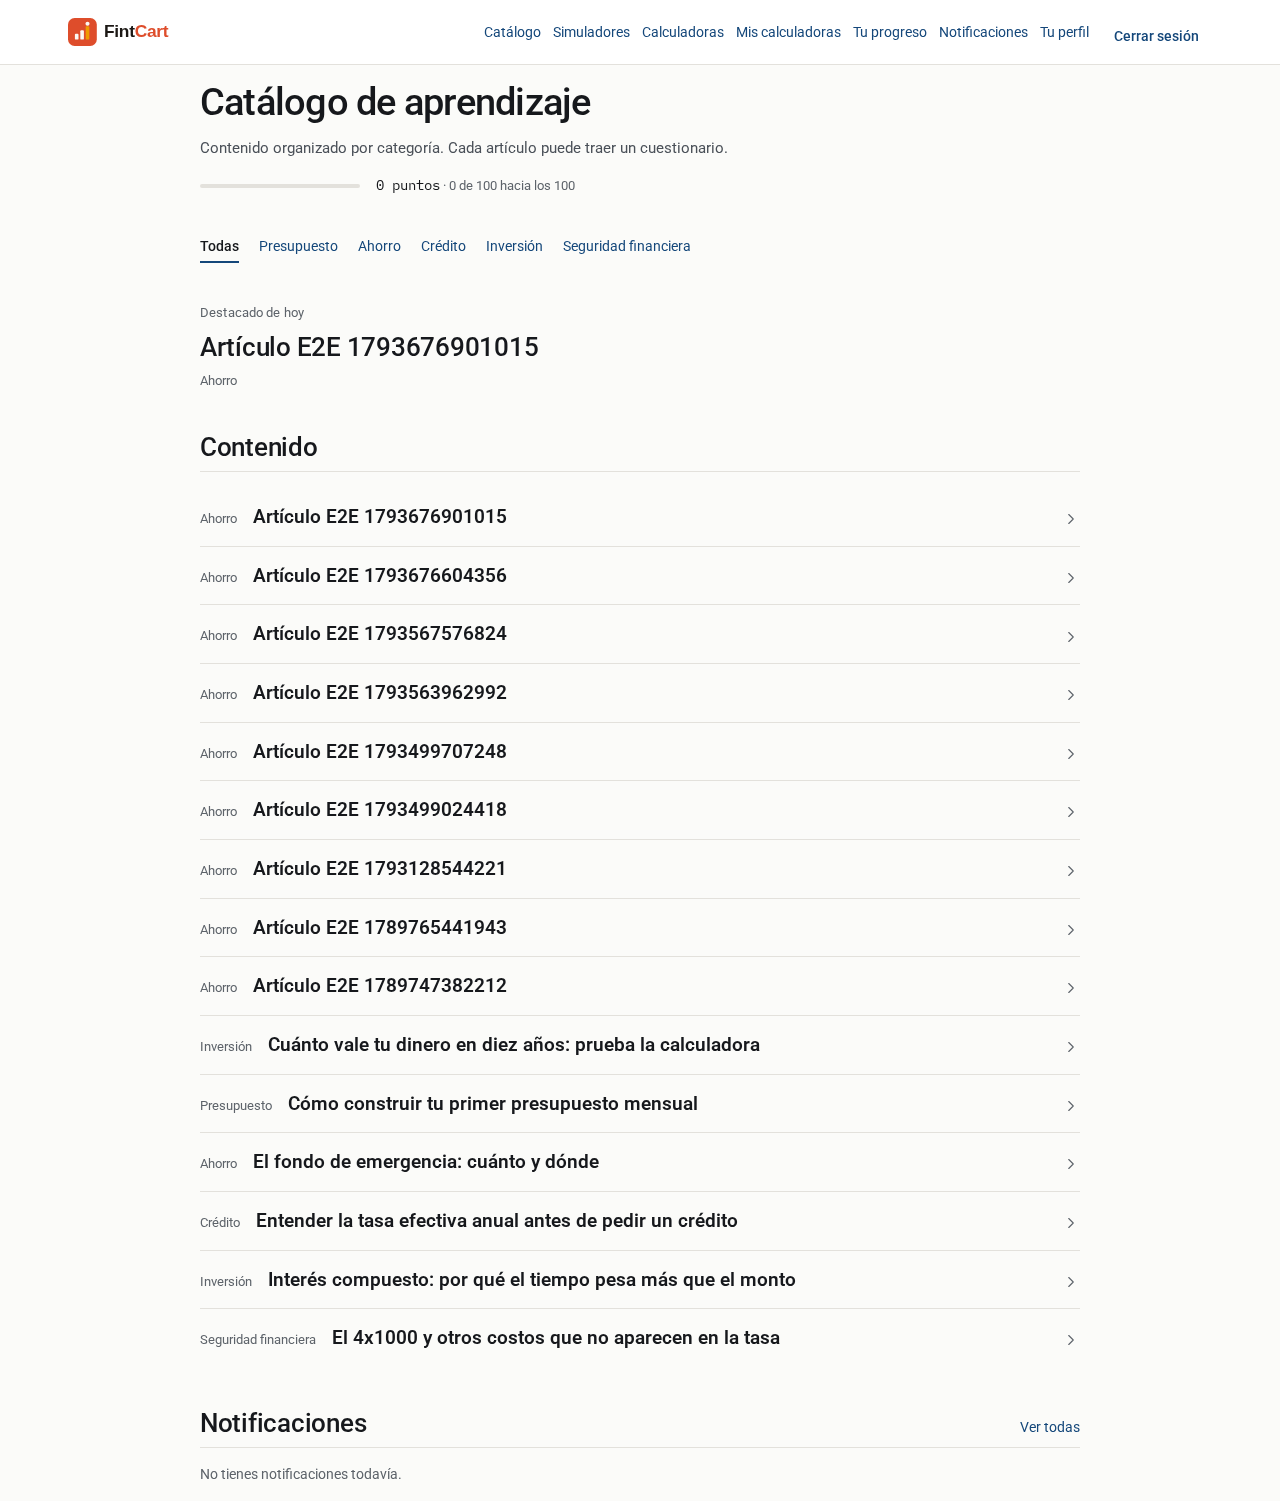
\includegraphics[width=0.78\linewidth]{fig-catalogo-1280}
  \caption{The catalog at 1280 px. Notice the single accent, the 880 px column, the silent
  left-hand index, and the one-pixel rules between article rows — the only chrome a list is
  allowed.}
  \label{fig:catalogo-1280}
\end{figure}

\begin{figure}[htbp]
  \centering
  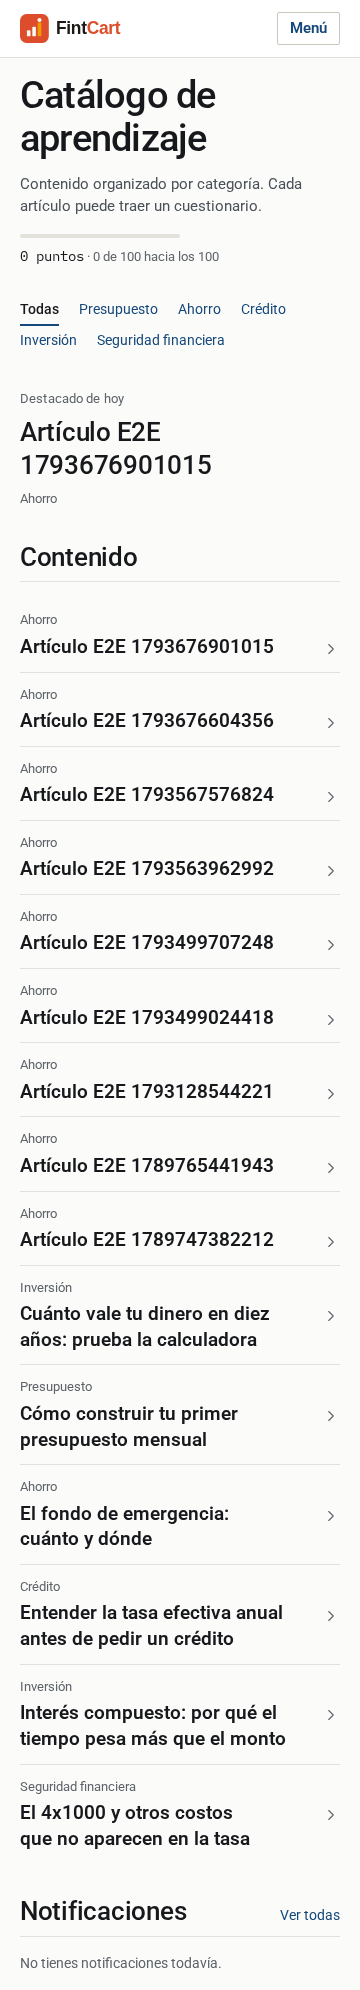
\includegraphics[height=0.78\textheight,keepaspectratio]{fig-catalogo-360}
  \caption{The same catalog at 360 px. The column reflows without horizontal overflow; the
  hierarchy survives because it is carried by type size and space, not by a grid that needs
  three zones to make sense.}
  \label{fig:catalogo-360}
\end{figure}

The access screen carries the same rule at its most consequential point. On a narrow phone the
obvious temptation is to hide the brand panel and leave only the form; doing so would return the
platform to the anonymous form this feature exists to correct, on the device where most people
arrive. So the panel degrades instead: under 768 px it becomes a compact top band with the
wordmark and title, sacrificing the subtitle and the three indicators (which repeat what the form
below already says), and it is never hidden. Figure~\ref{fig:login-480} shows why that matters —
a student on a 360 px phone still sees whose platform this is before typing a credential.

\begin{figure}[htbp]
  \centering
  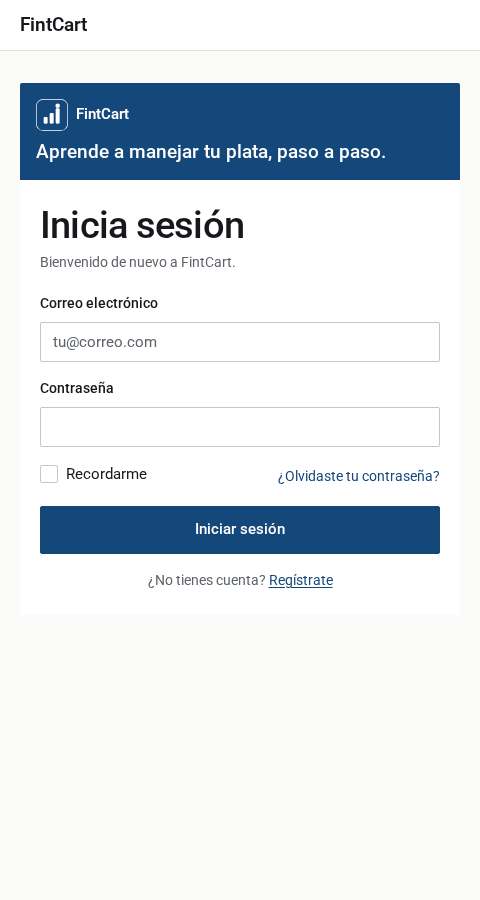
\includegraphics[width=0.62\linewidth]{fig-login-480}
  \caption{Login at 480 px. The brand panel has degraded to a compact band at the top rather than
  disappearing; the mark and wordmark remain the first thing a student reads.}
  \label{fig:login-480}
\end{figure}

\subsection{A monetary figure is never truncated}

The strongest constraint in the design is not visual at all, and it overrides every other layout
decision: a monetary figure is never truncated. Truncating \fcnum{\$1.234.567} to
\fcnum{\$1.234\ldots} is not incomplete text; it is a false datum, and it is the visual expression
of the platform's non-negotiable precision principle. The figure is rendered in the data face
(IBM Plex Mono) with tabular numerals and zero tracking, so a column of digits stays aligned and
the thousands separator is never mistaken for a decimal point. When a figure does not fit, the
design reduces the container or reflows the layout — it never clips or ellipsizes the number.
Below 768 px the result figure drops one type step precisely so the full amount keeps fitting
inside the 320 px of useful content. Figure~\ref{fig:resultado-1280} shows the result panel: the
monetary figure is the largest element on the screen and is drawn whole, in the data face, because
it is the one number on the page that must be exactly what the simulator service computed.

\begin{figure}[htbp]
  \centering
  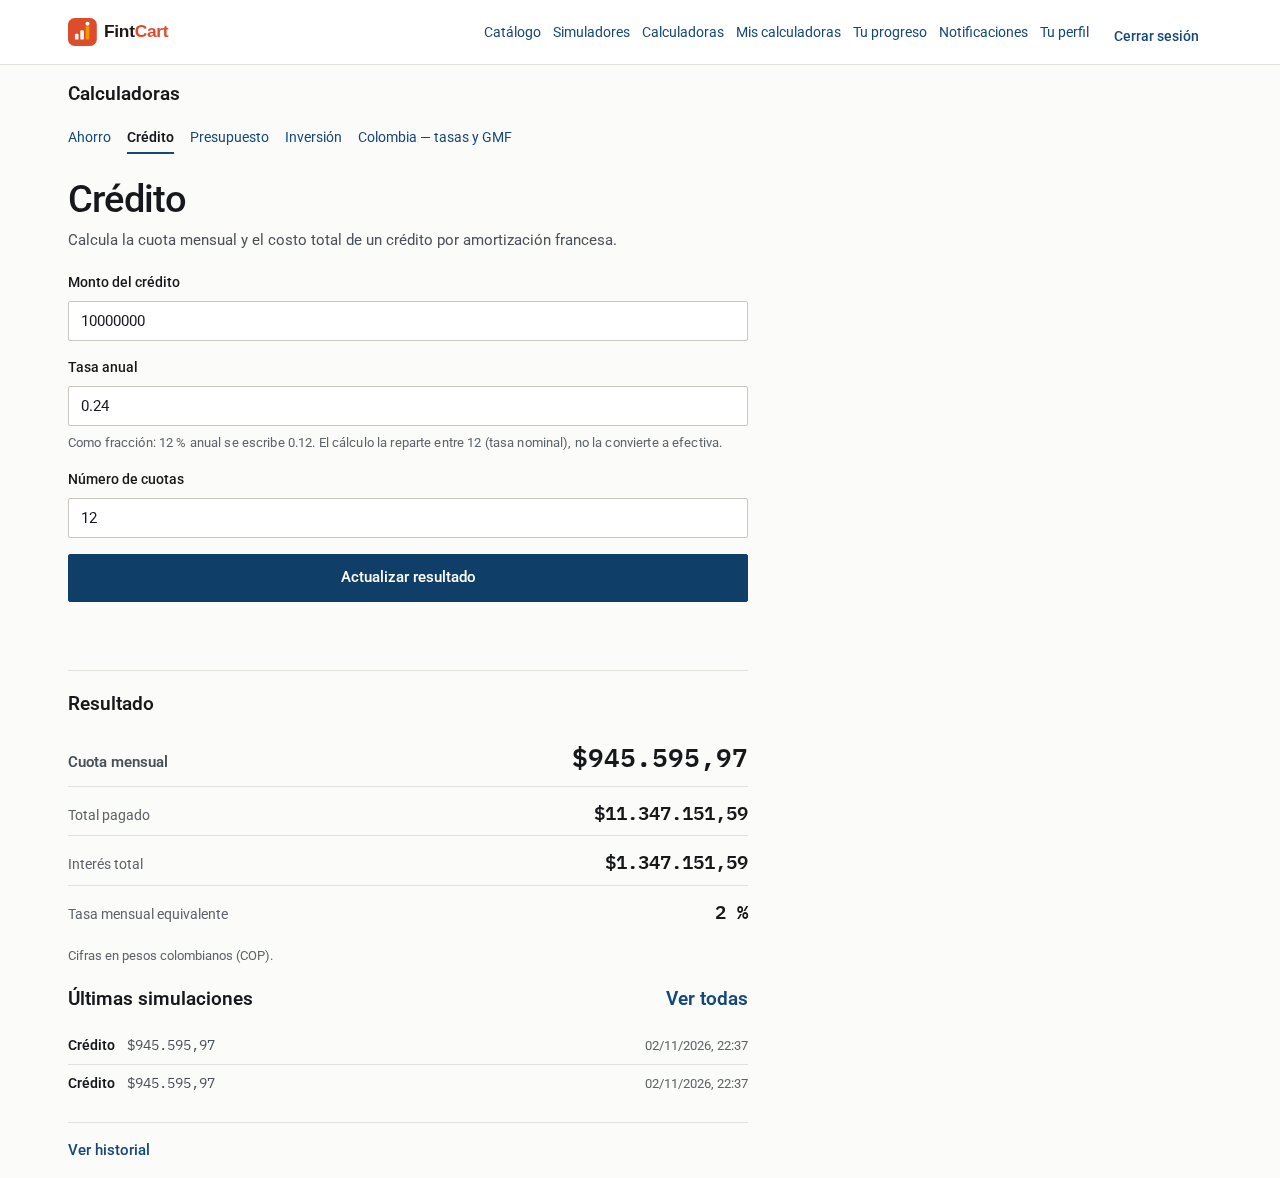
\includegraphics[width=0.78\linewidth]{fig-resultado-1280}
  \caption{Simulator result at 1280 px. The monetary figure is set in the data face with tabular
  numerals and rendered whole — the layout yields to the number, never the number to the layout.}
  \label{fig:resultado-1280}
\end{figure}

\subsection{What the redesign had to fight}

Four measured regressions summarize what the redesign actually contended with, and each one is a
lesson rather than an anecdote. The before/after probe comparison recorded uppercase eyebrows
falling from 32 to 0 and three-zone grids from 6 to 1: the first number proves the chrome was
systematic, and the second proves the single-column decision was a real reduction, not a
renaming. A four-pixel overflow at 360 px survived human review because it lived on
\code{/simuladores/colombia_especifica}, a route the ad hoc screenshot sweep never visited: a
sentence-length button label with \code{white-space: nowrap} measured 344 px inside a 320 px
column, and it could not shrink until the button primitive exposed a \code{--fc-btn-wrap} property
that lets a name — as opposed to an action — wrap. The lesson is that a one-digit overflow is
invisible to a person scrolling a screenshot and must be asserted, not looked at.

The deepest regression was in the token layer itself. The accessibility gate measured
\code{--text-muted} on the inset surface at 3.77:1, below the AA floor of 4.5:1, and later
\code{--fc-ink-3} on the accent tint at 4.38:1 while the token file's comment claimed 4.76:1.
The claim was true — against white. The token was used on a tinted surface. The comment now
records all four surfaces where text appears, and the fix darkened the ink rather than lightening
the tint, because lightening the tint would have broken the token on every surface darker than
paper. The lesson is the failure mode: a number in a source file that was true in one context and
false in the one that shipped, and that only measured, computed color could contradict.
Table~\ref{tab:lessons} collects the four.

\begin{table}[htbp]
  \centering
  \begin{tabular}{p{3.2cm}p{3.4cm}p{4.6cm}p{2.4cm}}
    \hline
    Regression & Before & After & Lesson \\
    \hline
    Uppercase eyebrows & 32 & 0 & Hierarchy must come from type, not from spaced caps \\
    Three-zone grids & 6 & 1 & A single column is a reduction, not a restyle \\
    360 px overflow & 344 px label in a 320 px column & \code{--fc-btn-wrap} lets names wrap & Overflow must be asserted, not eyeballed \\
    Token contrast & 3.77:1 inset; 4.38:1 on tint (claimed 4.76:1) & \code{--fc-ink-3} darkened to \texttt{\#5D636A} & Measure against the surface in use, not against white \\
    \hline
  \end{tabular}
  \caption{The four regressions the redesign had to fight, each reduced to its before, its after,
  and the design lesson it carries.}
  \label{tab:lessons}
\end{table}

\subsection{Accessibility as a testable property}

The design treats accessibility as something a machine can check, not something a reviewer
promises. Concretely, AA means two numbers: a contrast ratio of at least 4.5:1 for normal text and
3:1 for text at least 24 px or bold at least 19 px, measured on the computed color of the text and
its actual background — not on the value written in the token file. The end-to-end suite is the
enforcement point: it selects controls by role and accessible name in 110 of its 112 assertions,
which is why it survives a full redesign and fails the moment that redesign breaks the
accessibility it selects by. Two defects that the suite caught show what this buys.

The first was an unnamed \code{role="progressbar"}: a screen reader announcing \enquote{progress
bar} can say nothing about which progress, so the primitive now derives its accessible name from
an explicit label or from the visible text beside the bar, and both paths write the same
\code{aria-label}. The second was the \enquote{Regístrate} link on the login screen: it was
distinguishable from the sentence around it only by color, at 1.92:1, which fails WCAG 1.4.1 and
vanishes entirely under forced colors. The fix was the minimum that satisfies the criterion — an
underline on links inside prose, which survives forced color modes without turning the link into a
button. The same suite, run at five widths, is also what holds the 360 px floor and the
never-hidden brand panel in place: those are not design opinions, they are assertions that fail
the build.

The one boundary the feature did not cross is the editorial screen. It migrated only the frame —
the header, the side panels, the publication states — and left the writing surface to
feature 002, which owns it. Figure~\ref{fig:editorial-1280} shows the
result: the frame already speaks the same design language as the rest of the platform, while the
surface it surrounds is deliberately out of scope for this feature.

\begin{figure}[htbp]
  \centering
  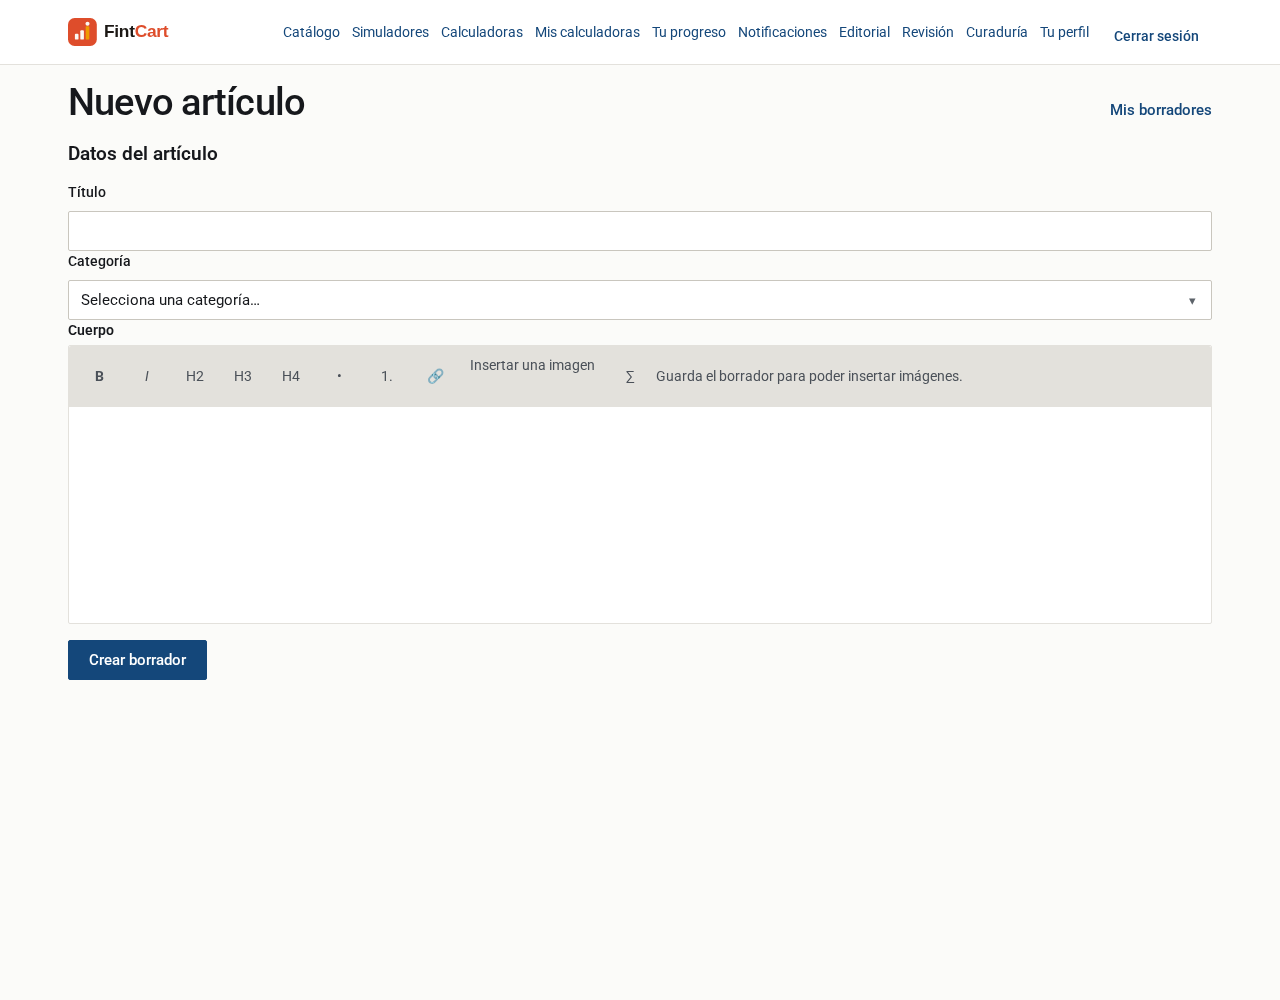
\includegraphics[width=0.78\linewidth]{fig-editorial-1280}
  \caption{The editorial frame at 1280 px. Only the surrounding chrome was migrated to the design
  system; the writing surface at its center belongs to feature 002 and was left untouched.}
  \label{fig:editorial-1280}
\end{figure}

% DONE: the design argument — institutional calm as a decision under constraint, the checkable
% token layer, the 19 primitives with a layer retired instead of added, the single responsive
% scale, the never-truncated monetary figure, the regressions as design lessons, and accessibility
% as a testable property.
